\documentclass[11pt,a4paper]{article}

% ── Packages ──
\usepackage[margin=2.5cm]{geometry}
\usepackage{amsmath, amssymb}
\usepackage{graphicx}
\usepackage{booktabs}
\usepackage{siunitx}
\usepackage{float}
\usepackage{hyperref}
\usepackage{caption}
\usepackage{subcaption}

% ── Placeholder command ──
\newcommand{\placeholder}[1]{\textbf{[#1]}}

% ── Title ──
\title{Noise Floor Estimation of a Current Amplifier}
\author{
  \placeholder{Student Name 1} \\
  \placeholder{Student Name 2} \\
  \placeholder{Student Name 3} \\[1em]
  \placeholder{Department, Seoul National University}
}
\date{\placeholder{Experiment Date}}

\begin{document}
\maketitle

% ============================================================
\section{Introduction}
% ============================================================

In precision current measurements, the noise floor of the measurement system
determines the minimum detectable signal. This experiment characterizes the
noise floor of a current amplifier by measuring the output voltage noise
with open-circuit input for two different cable lengths. Since the dominant
noise source is expected to be the cable capacitance coupled with the
amplifier's input voltage noise, the noise should scale linearly with cable
length. By comparing measurements from two cables with an approximately
$2\times$ length ratio, we verify this prediction.

% ============================================================
\section{Theory}
% ============================================================

\subsection{Current Amplifier Circuit}

The current amplifier consists of an operational amplifier with a feedback
resistor $R_f$. A sample (device under test) with resistance $R_s$ is
connected to the inverting input via a coaxial cable of capacitance $C_s$.
The transimpedance gain is:
\begin{equation}
  \text{Gain} = R_f \quad [\si{V/A}]
\end{equation}

\noindent Experimental parameters (fill in actual values):
\begin{itemize}
  \item Feedback resistor: $R_f = $ \placeholder{Rf} $\si{\ohm}$
  \item Sample resistance: $R_s = $ \placeholder{Rs} $\si{\ohm}$ (open circuit $\to \infty$)
  \item Gain setting: \placeholder{Gain} $\si{V/A}$
  \item Cable capacitance per meter: $\sim \SI{100}{pF/m}$
  \item Long cable length: \placeholder{L-long} $\si{m}$,
        $C_s^{\text{long}} = $ \placeholder{Cs-long} $\si{pF}$
  \item Short cable length: \placeholder{L-short} $\si{m}$,
        $C_s^{\text{short}} = $ \placeholder{Cs-short} $\si{pF}$
  \item Op-amp current noise: $i_n \approx \SI{5}{fA/\sqrt{Hz}}$
  \item Op-amp voltage noise: $e_n \approx \SI{3}{nV/\sqrt{Hz}}$
\end{itemize}

\subsection{Noise Sources}

The total equivalent input current noise spectral density has contributions from:

\begin{enumerate}
  \item \textbf{Op-amp current noise}: $i_n$
  \item \textbf{Thermal noise from sample}: $\sqrt{4 k_B T / R_s}$
  \item \textbf{Thermal noise from feedback resistor}: $\sqrt{4 k_B T / R_f}$
  \item \textbf{Voltage noise through sample}: $e_n / R_s$
  \item \textbf{Capacitance noise} (dominant): $e_n \cdot 2\pi f \cdot C_s$
\end{enumerate}

The total current noise spectral density is:
\begin{equation}
  \tilde{i}_{n,\text{total}}^2(f) = i_n^2 + \frac{4 k_B T}{R_s}
    + \frac{4 k_B T}{R_f}
    + \left(\frac{e_n}{R_s}\right)^2
    + \left(e_n \cdot 2\pi f \cdot C_s\right)^2
  \label{eq:noise_total}
\end{equation}

For an open-circuit measurement ($R_s \to \infty$), the sample-related terms
vanish, leaving:
\begin{equation}
  \tilde{i}_{n,\text{total}}^2(f) \approx i_n^2
    + \frac{4 k_B T}{R_f}
    + \left(e_n \cdot 2\pi f \cdot C_s\right)^2
  \label{eq:noise_open}
\end{equation}

The RMS input current noise integrated over the measurement bandwidth $f_M$ is:
\begin{equation}
  i_{n,\text{rms}} = \sqrt{\int_0^{f_M} \tilde{i}_{n,\text{total}}^2(f)\, df}
\end{equation}

The measured RMS voltage noise at the amplifier output is:
\begin{equation}
  \Delta V_{\text{rms}} = i_{n,\text{rms}} \times \text{Gain}
  \label{eq:Vrms}
\end{equation}

\subsection{Cable Length Dependence}

Since the capacitance noise term dominates at higher frequencies and
$C_s \propto L$ (cable length), the integrated noise scales approximately as:
\begin{equation}
  \Delta V_{\text{rms}} \propto C_s \propto L
\end{equation}
Therefore, doubling the cable length should approximately double the output noise.

% ============================================================
\section{Experimental Setup}
% ============================================================

\placeholder{Describe the experimental setup: current amplifier model,
oscilloscope/DAQ used, sampling rate, measurement duration, temperature, etc.}

Two coaxial cables of different lengths were used:
\begin{itemize}
  \item \textbf{Long cable}: \placeholder{L-long} $\si{m}$
  \item \textbf{Short cable}: \placeholder{L-short} $\si{m}$
        (approximately half the long cable length)
\end{itemize}

For each cable, 5 independent measurements were recorded with open-circuit
input (no sample connected). Each measurement consists of a voltage time
trace $V(t)$ sampled at \placeholder{sampling rate} with \placeholder{N}
data points, corresponding to a total measurement time of
$\sim\SI{10}{ms}$.

% ============================================================
\section{Results}
% ============================================================

\subsection{Time-Domain Traces}

Figure~\ref{fig:overlay} shows the overlay of all 5 measurements for each
cable length. The long cable traces show visibly larger voltage fluctuations.

\begin{figure}[H]
  \centering
  \begin{subfigure}[b]{0.48\textwidth}
    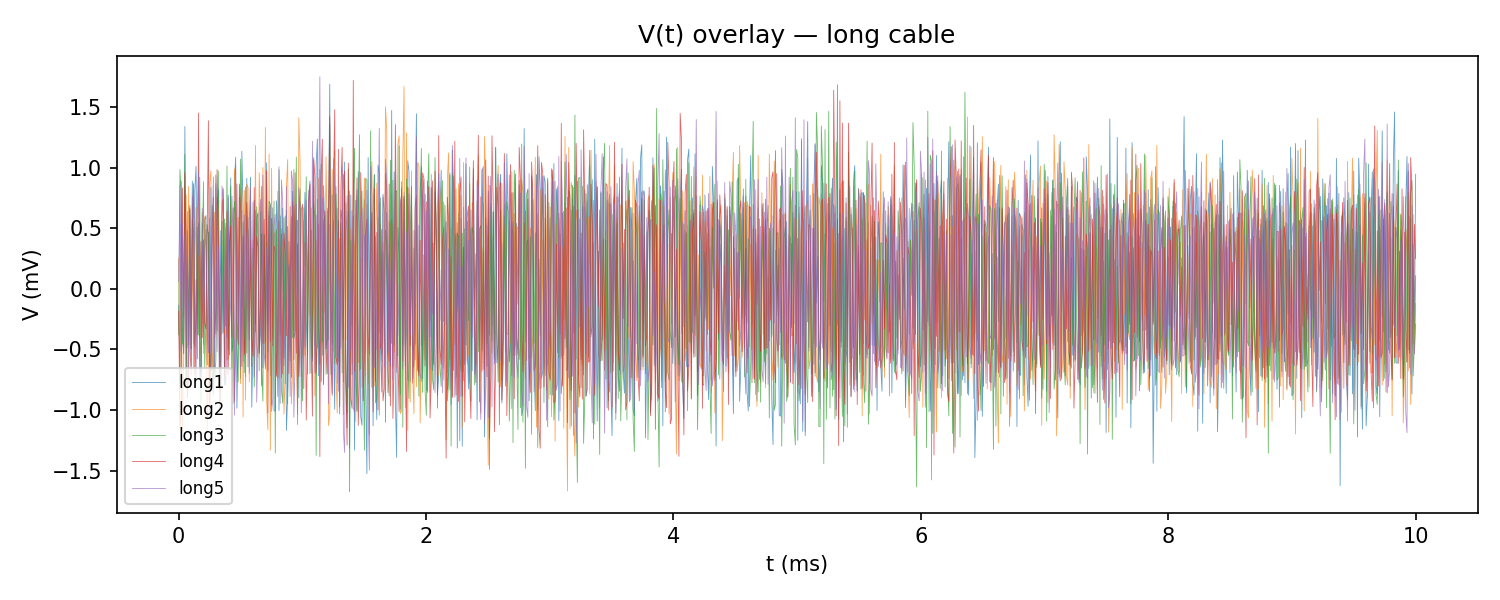
\includegraphics[width=\textwidth]{../images/long_overlay.png}
    \caption{Long cable}
  \end{subfigure}
  \hfill
  \begin{subfigure}[b]{0.48\textwidth}
    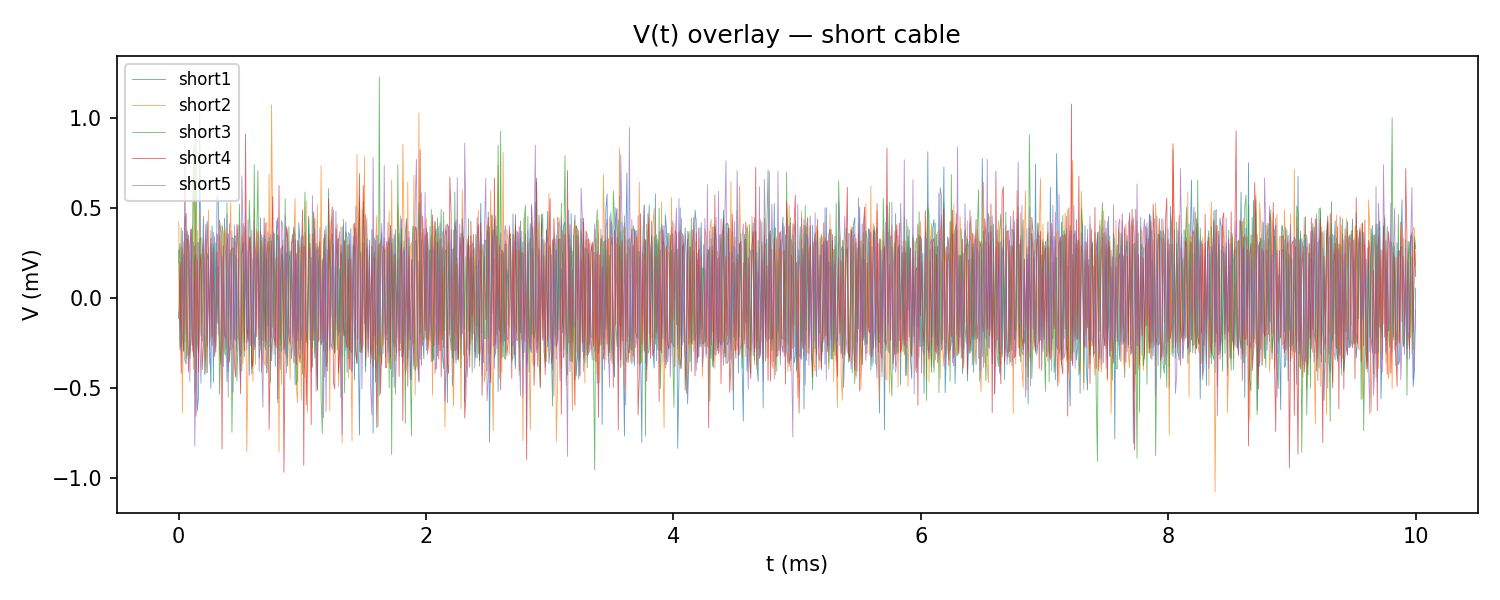
\includegraphics[width=\textwidth]{../images/short_overlay.png}
    \caption{Short cable}
  \end{subfigure}
  \caption{Overlay of $V(t)$ traces for (a) long and (b) short cable.}
  \label{fig:overlay}
\end{figure}

\subsection{Voltage Statistics}

Table~\ref{tab:stats} summarizes the mean and standard deviation of the
measured voltage for each trial.

\begin{table}[H]
  \centering
  \caption{Voltage noise statistics for each measurement.}
  \label{tab:stats}
  \begin{tabular}{lSS}
    \toprule
    {Label} & {Mean (\si{mV})} & {Std.\ Dev.\ (\si{mV})} \\
    \midrule
    long1  & 0.0167 & 0.7446 \\
    long2  & 0.0277 & 0.7033 \\
    long3  & 0.0035 & 0.7282 \\
    long4  & 0.0213 & 0.7071 \\
    long5  & 0.0314 & 0.6900 \\
    \midrule
    short1 & 0.0022 & 0.3483 \\
    short2 & 0.0145 & 0.3654 \\
    short3 & 0.0226 & 0.3553 \\
    short4 & 0.0098 & 0.3587 \\
    short5 & 0.0344 & 0.3559 \\
    \bottomrule
  \end{tabular}
\end{table}

\noindent Group-averaged standard deviations and their ratio:
\begin{align}
  \sigma_{\text{long}}  &= \SI{0.7147}{mV} \notag \\
  \sigma_{\text{short}} &= \SI{0.3567}{mV} \notag \\
  \frac{\sigma_{\text{long}}}{\sigma_{\text{short}}} &= 2.003
  \label{eq:ratio}
\end{align}

\subsection{Power Spectral Density}

Figure~\ref{fig:psd} shows the averaged power spectral density (PSD) for
each cable group. The PSD of the long cable is consistently higher,
particularly at higher frequencies where the $f^2$-dependent capacitance
noise term dominates.

\begin{figure}[H]
  \centering
  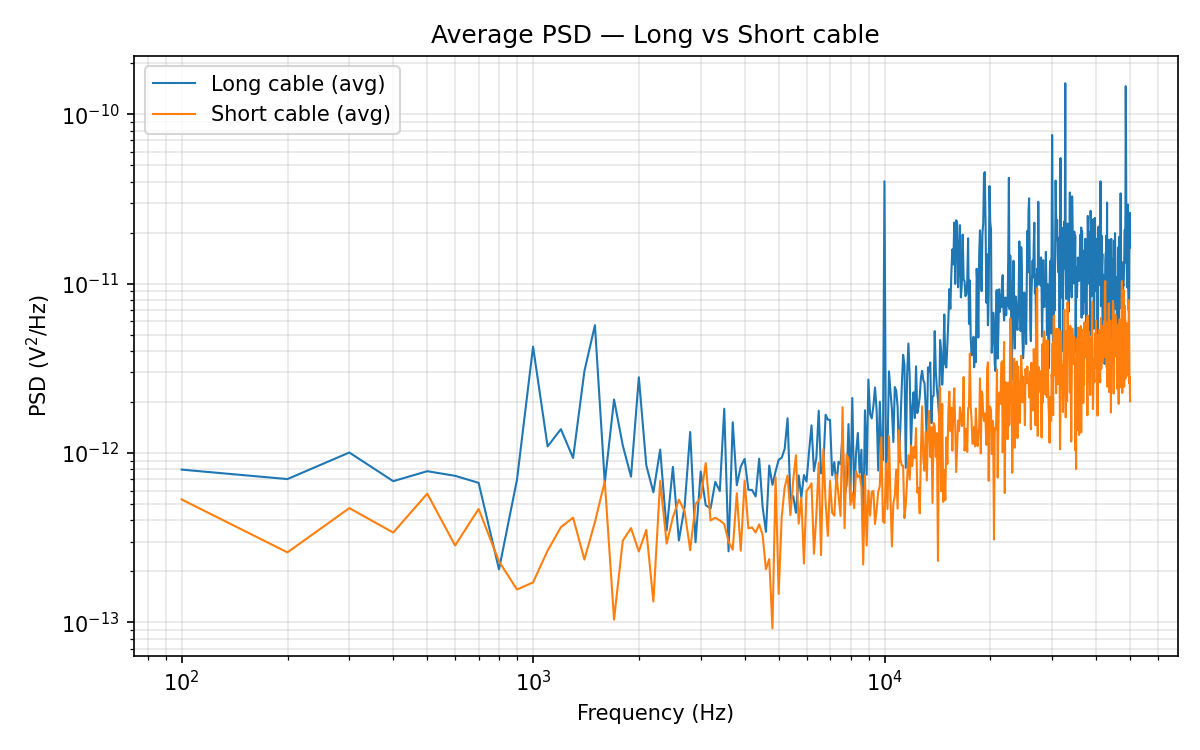
\includegraphics[width=0.75\textwidth]{../images/psd_comparison.png}
  \caption{Averaged PSD for long vs.\ short cable. The separation increases
           with frequency, consistent with the $C_s$-dependent noise term.}
  \label{fig:psd}
\end{figure}

\subsection{Voltage Distribution}

Figure~\ref{fig:hist} shows the histogram of all voltage samples for each
cable group. Both distributions are approximately Gaussian (as expected for
thermal/amplifier noise), with the long cable distribution being broader.

\begin{figure}[H]
  \centering
  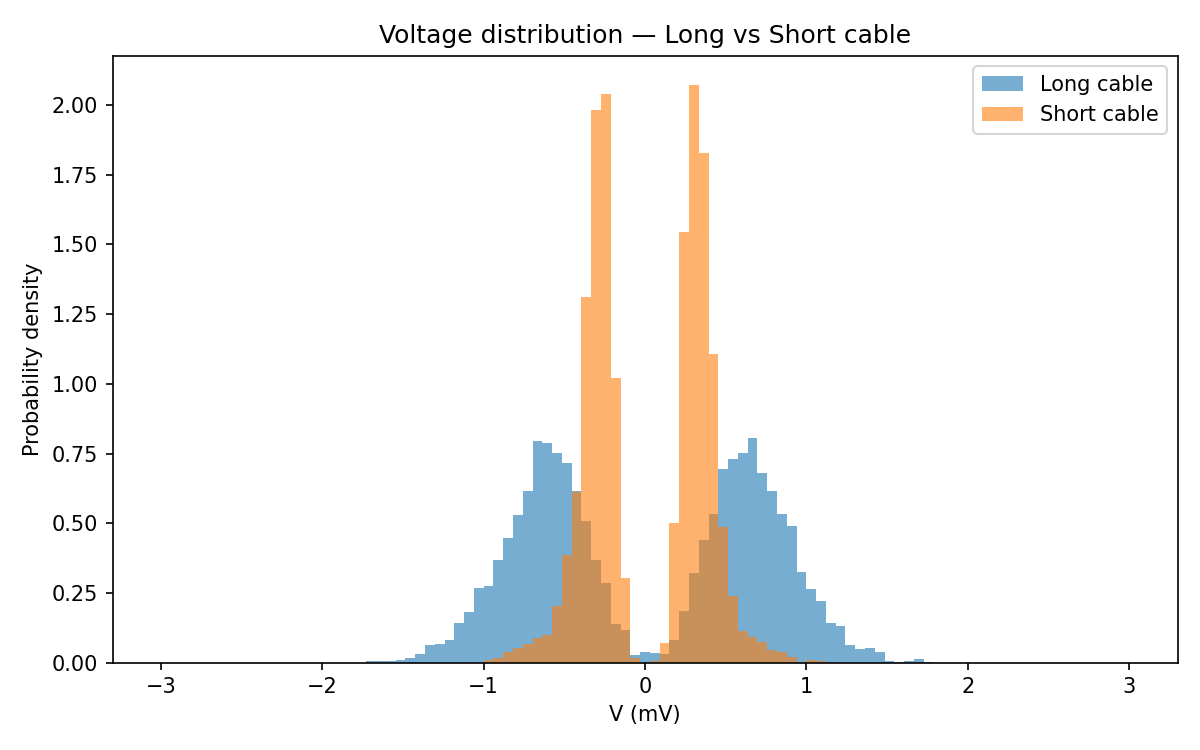
\includegraphics[width=0.65\textwidth]{../images/histogram_comparison.png}
  \caption{Voltage distribution for long and short cable measurements.}
  \label{fig:hist}
\end{figure}

% ============================================================
\section{Discussion}
% ============================================================

\subsection{Verification of Linear Scaling}

The measured noise ratio $\sigma_{\text{long}} / \sigma_{\text{short}} = 2.003$
is in excellent agreement with the expected ratio of $\sim 2$ based on the
cable length ratio $L_{\text{long}} / L_{\text{short}} \approx 2$. This
confirms that the dominant noise source is the cable capacitance term
$e_n \cdot 2\pi f \cdot C_s$ in Eq.~\eqref{eq:noise_open}.

\subsection{Theoretical Noise Estimate}

Using the parameters from the experimental setup, the theoretical RMS
voltage noise can be estimated. For the dominant capacitance term with
bandwidth $f_M = $ \placeholder{fM} $\si{Hz}$:

\begin{equation}
  i_{n,\text{cap,rms}} = e_n \cdot 2\pi C_s \sqrt{\frac{f_M^3}{3}}
\end{equation}

\begin{equation}
  \Delta V_{\text{rms,theory}} = i_{n,\text{cap,rms}} \times \text{Gain}
    = \text{\placeholder{value}}~\si{mV}
\end{equation}

\placeholder{Compare with measured sigma-long and sigma-short and discuss agreement/discrepancy.}

\subsection{Dominant Noise Source}

The PSD comparison (Fig.~\ref{fig:psd}) shows increasing separation between
the two curves at higher frequencies. This $f^2$ dependence in the PSD is
the signature of the capacitance noise term $(e_n \cdot 2\pi f \cdot C_s)^2$,
confirming it as the dominant noise contributor. The frequency-independent
terms ($i_n^2$, $4k_BT/R_f$) contribute a flat noise floor that is common
to both cable lengths.

% ============================================================
\section{Conclusion}
% ============================================================

We measured the noise floor of a current amplifier using two coaxial cables
with approximately $2\times$ length difference. The measured RMS voltage
noise ratio of $2.003$ between the long and short cables confirms the
theoretical prediction that the dominant noise source is the cable
capacitance coupled with the amplifier's input voltage noise ($e_n \cdot
2\pi f \cdot C_s$). This result demonstrates that minimizing cable
capacitance (i.e., using shorter cables) is critical for reducing the noise
floor in high-sensitivity current measurements.

% ============================================================
\newpage
\section*{Appendix: Individual Measurement Plots}
% ============================================================

\begin{figure}[H]
  \centering
  \begin{subfigure}[b]{0.48\textwidth}
    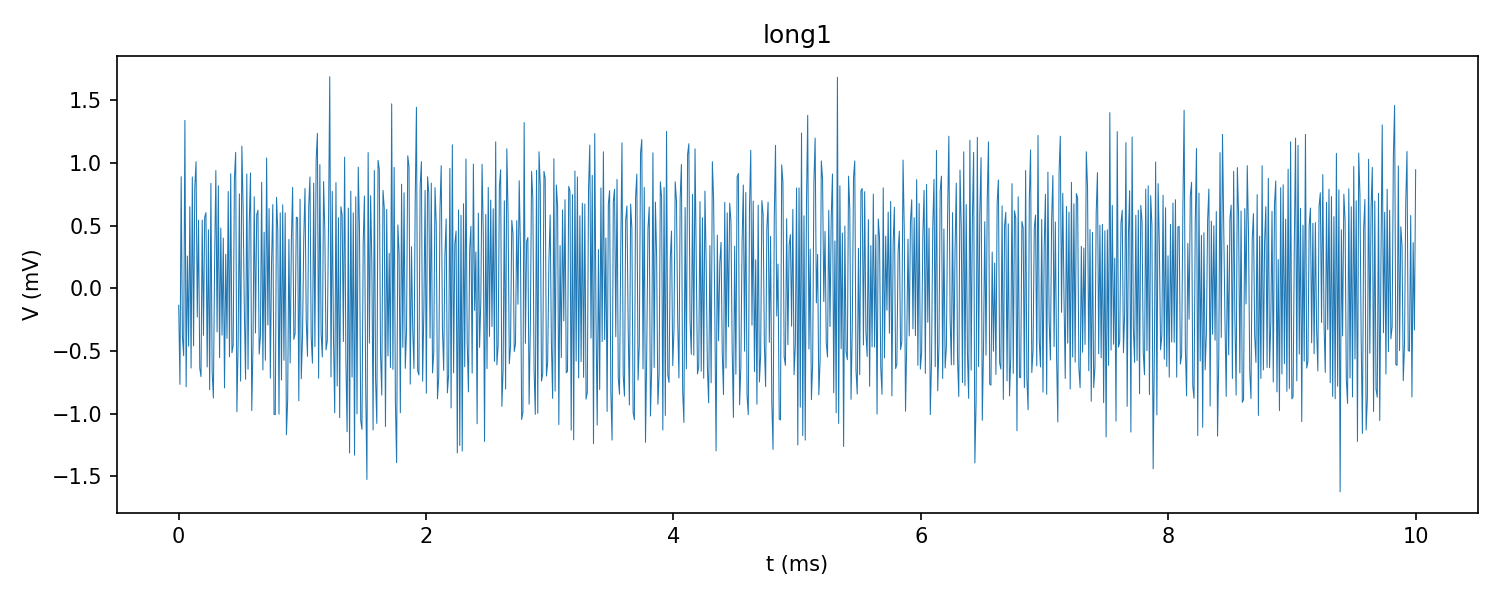
\includegraphics[width=\textwidth]{../images/long1.png}
    \caption{long1}
  \end{subfigure}\hfill
  \begin{subfigure}[b]{0.48\textwidth}
    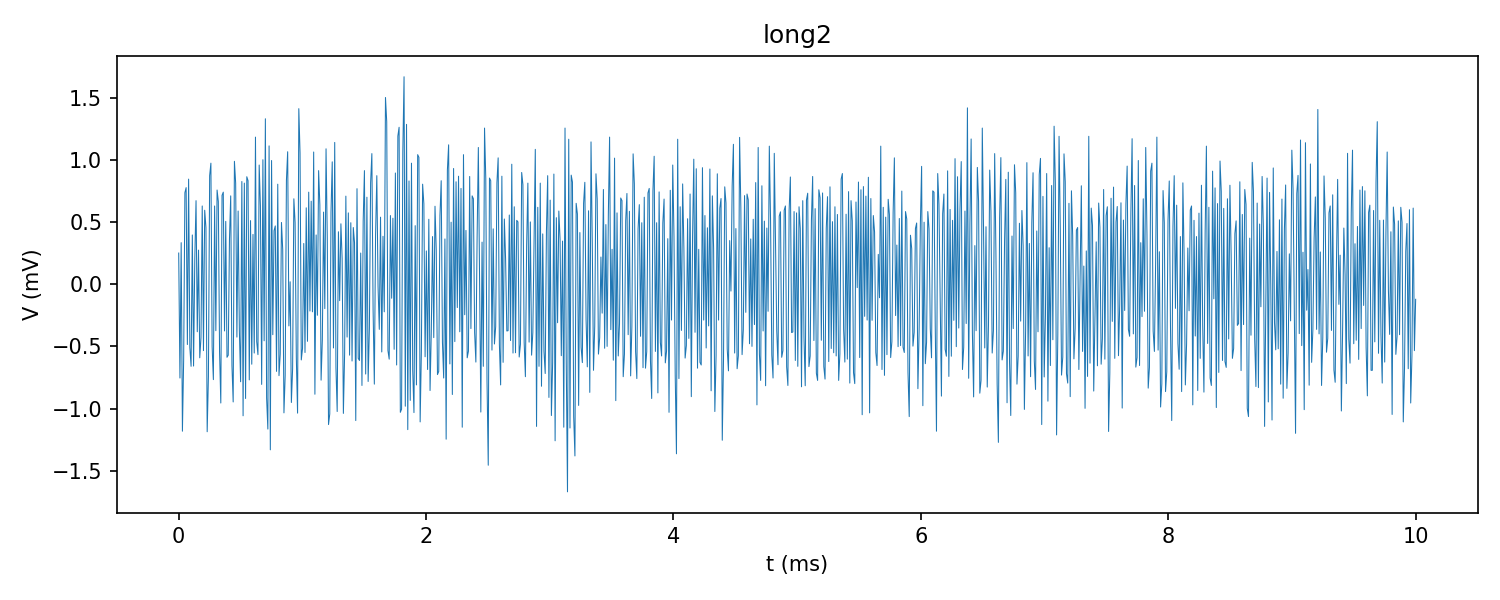
\includegraphics[width=\textwidth]{../images/long2.png}
    \caption{long2}
  \end{subfigure}\\[1em]
  \begin{subfigure}[b]{0.48\textwidth}
    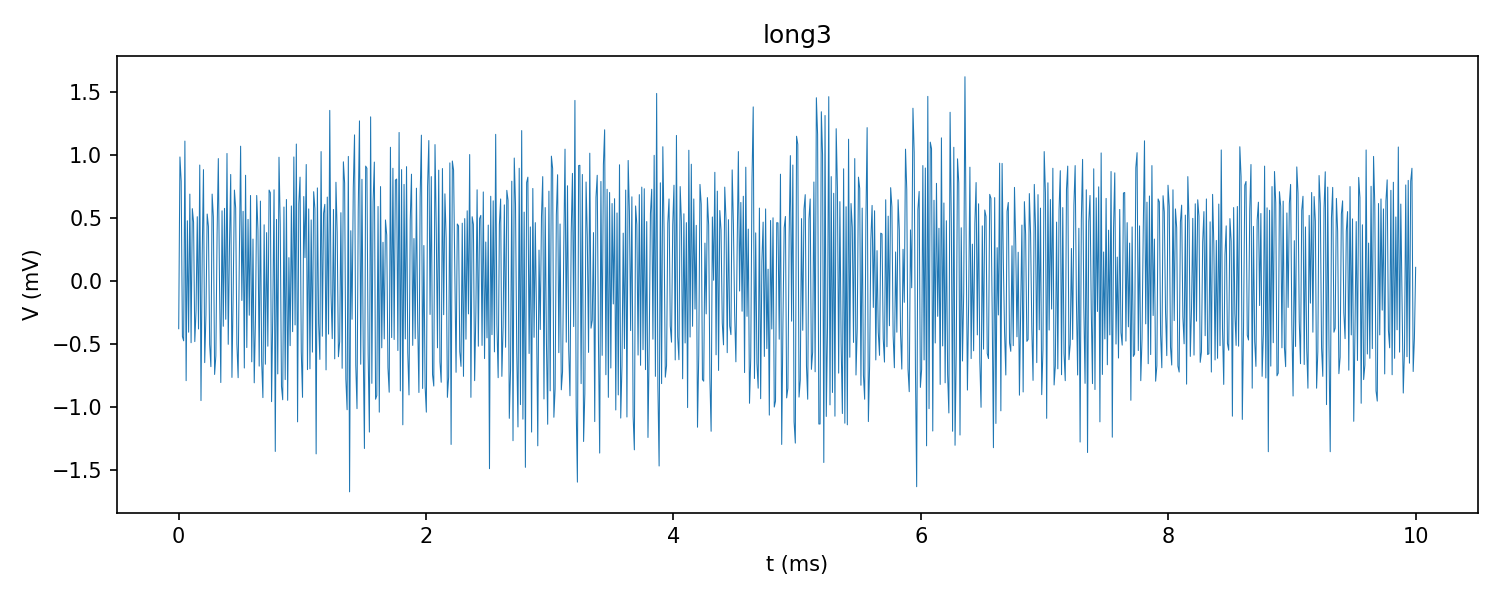
\includegraphics[width=\textwidth]{../images/long3.png}
    \caption{long3}
  \end{subfigure}\hfill
  \begin{subfigure}[b]{0.48\textwidth}
    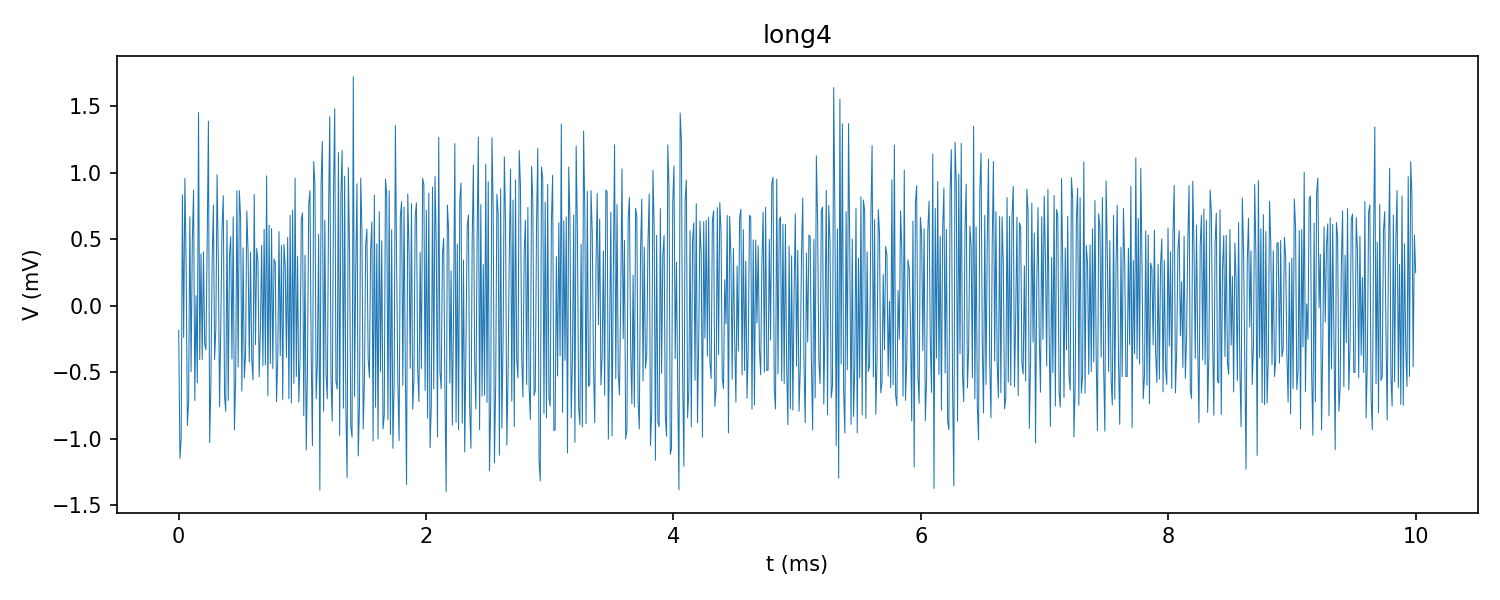
\includegraphics[width=\textwidth]{../images/long4.png}
    \caption{long4}
  \end{subfigure}\\[1em]
  \begin{subfigure}[b]{0.48\textwidth}
    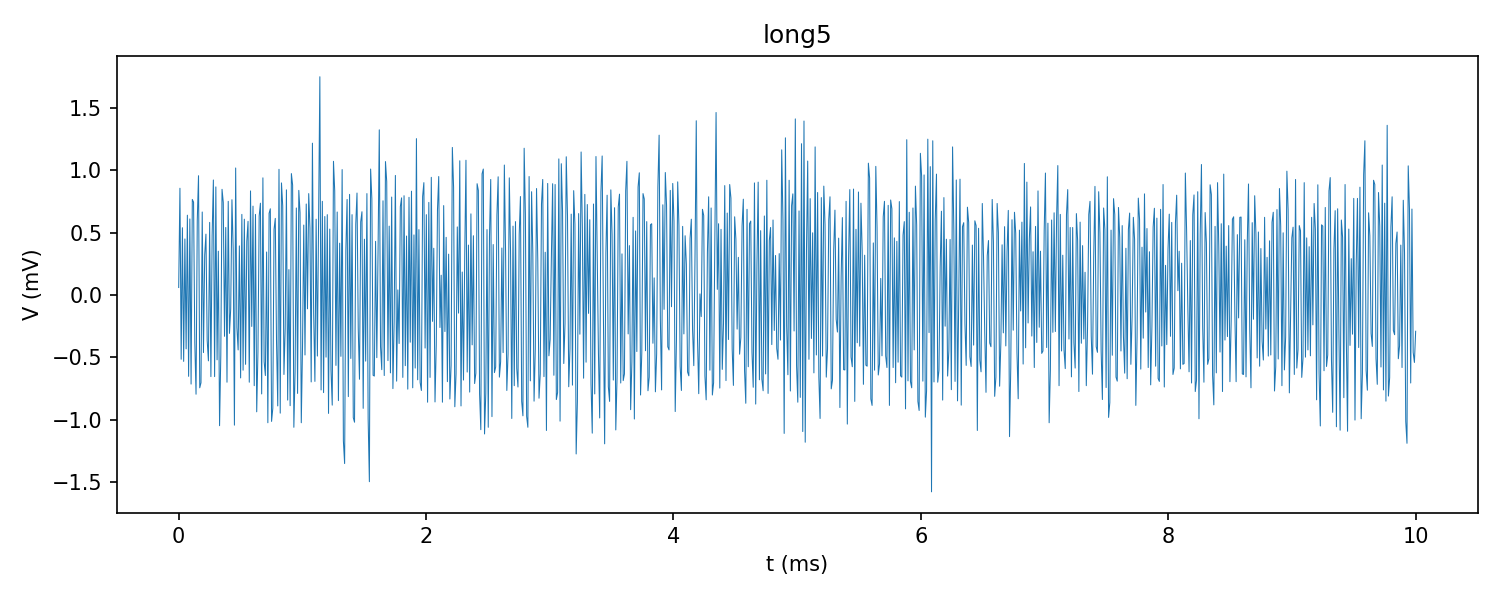
\includegraphics[width=\textwidth]{../images/long5.png}
    \caption{long5}
  \end{subfigure}
  \caption{Individual $V(t)$ traces for long cable measurements.}
\end{figure}

\begin{figure}[H]
  \centering
  \begin{subfigure}[b]{0.48\textwidth}
    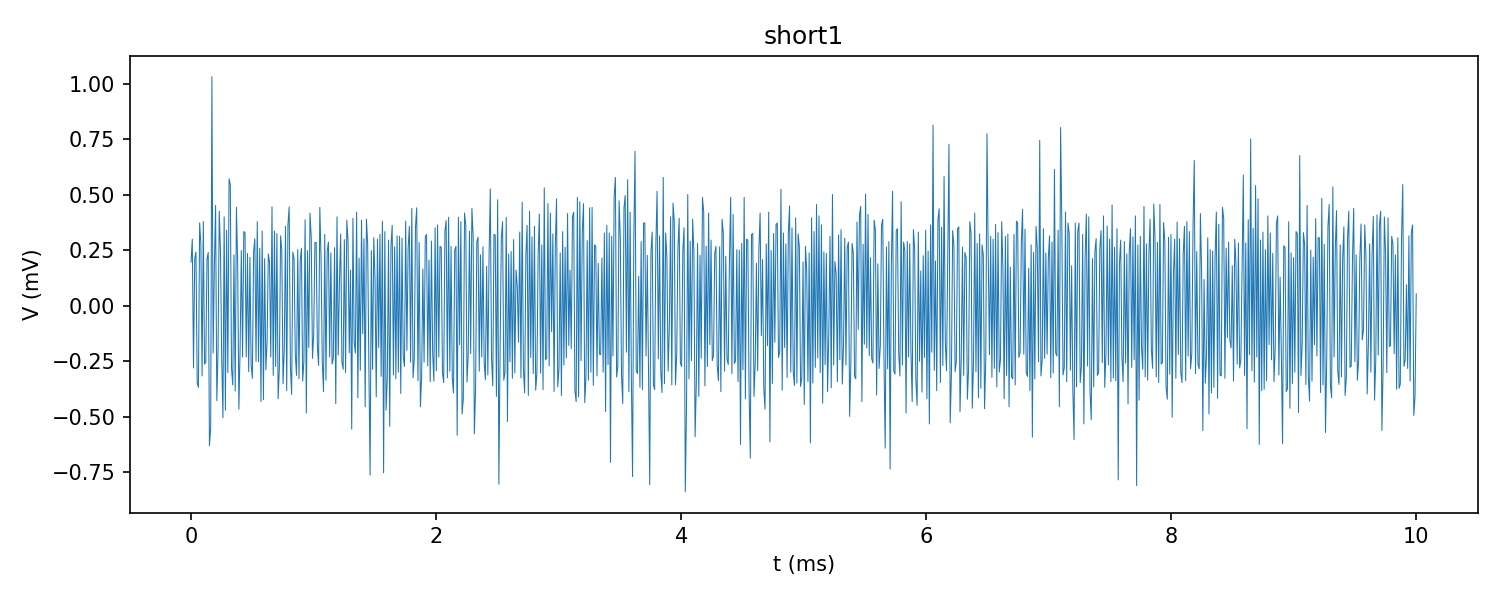
\includegraphics[width=\textwidth]{../images/short1.png}
    \caption{short1}
  \end{subfigure}\hfill
  \begin{subfigure}[b]{0.48\textwidth}
    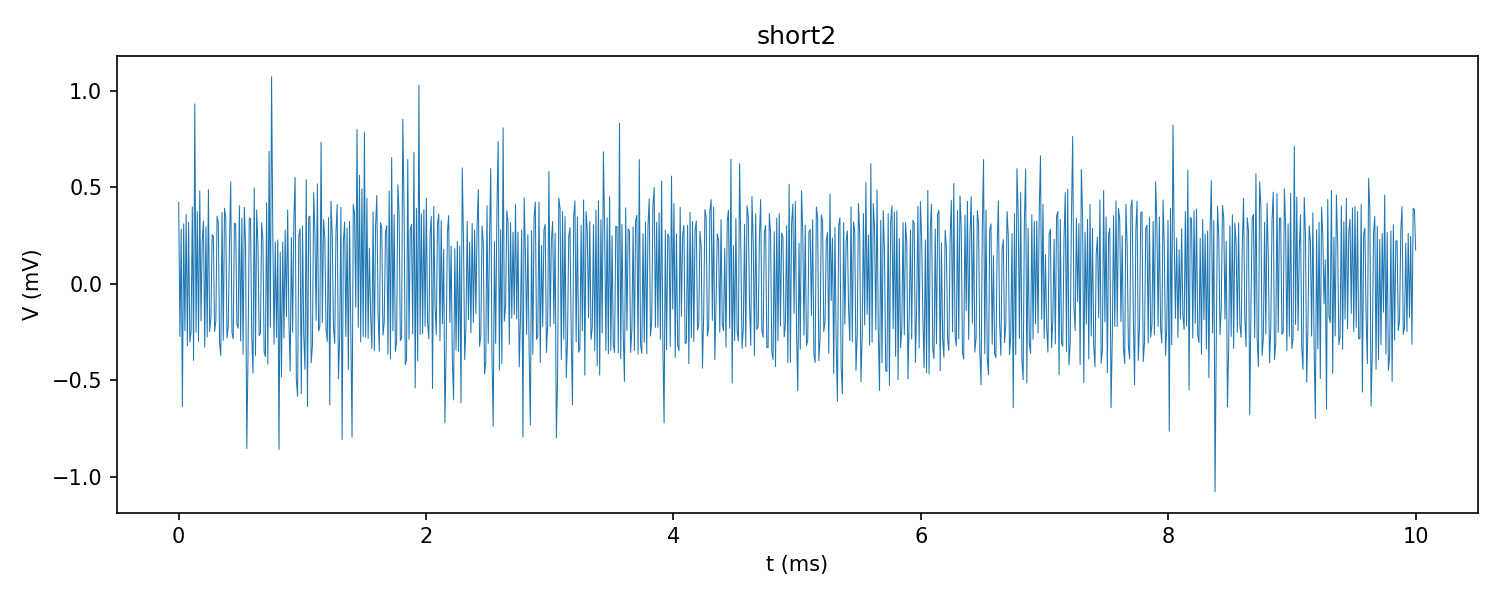
\includegraphics[width=\textwidth]{../images/short2.png}
    \caption{short2}
  \end{subfigure}\\[1em]
  \begin{subfigure}[b]{0.48\textwidth}
    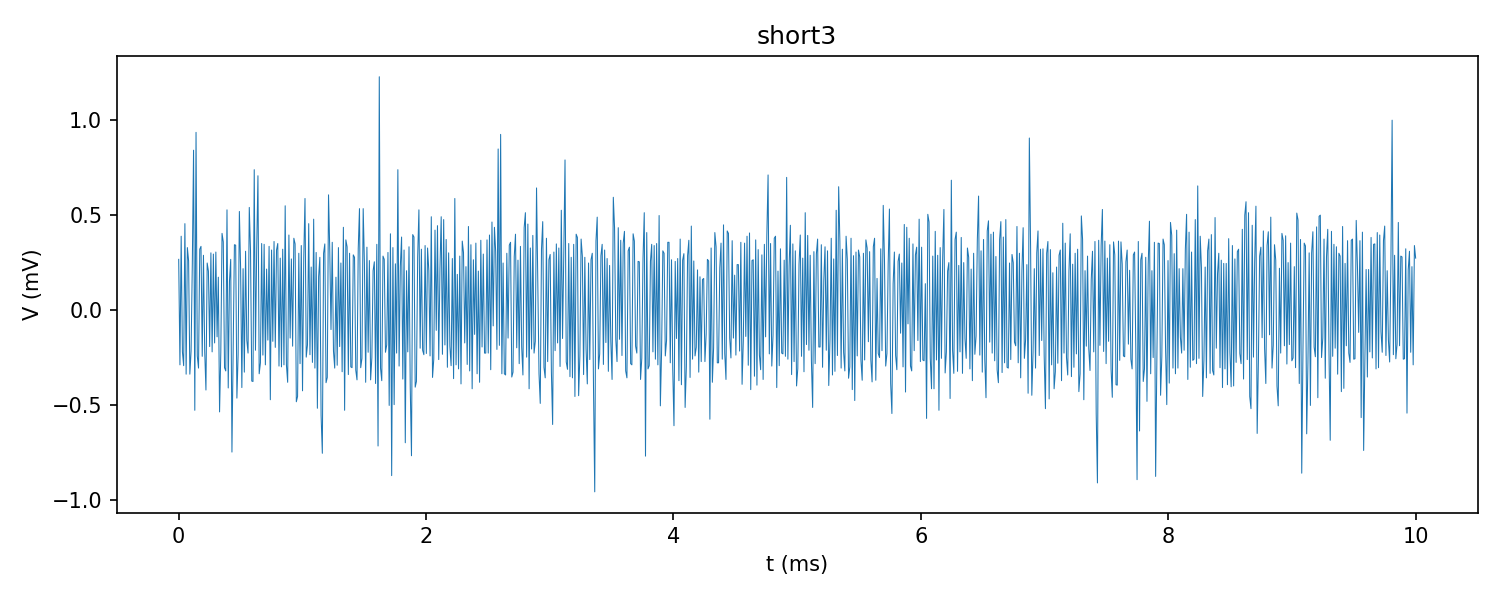
\includegraphics[width=\textwidth]{../images/short3.png}
    \caption{short3}
  \end{subfigure}\hfill
  \begin{subfigure}[b]{0.48\textwidth}
    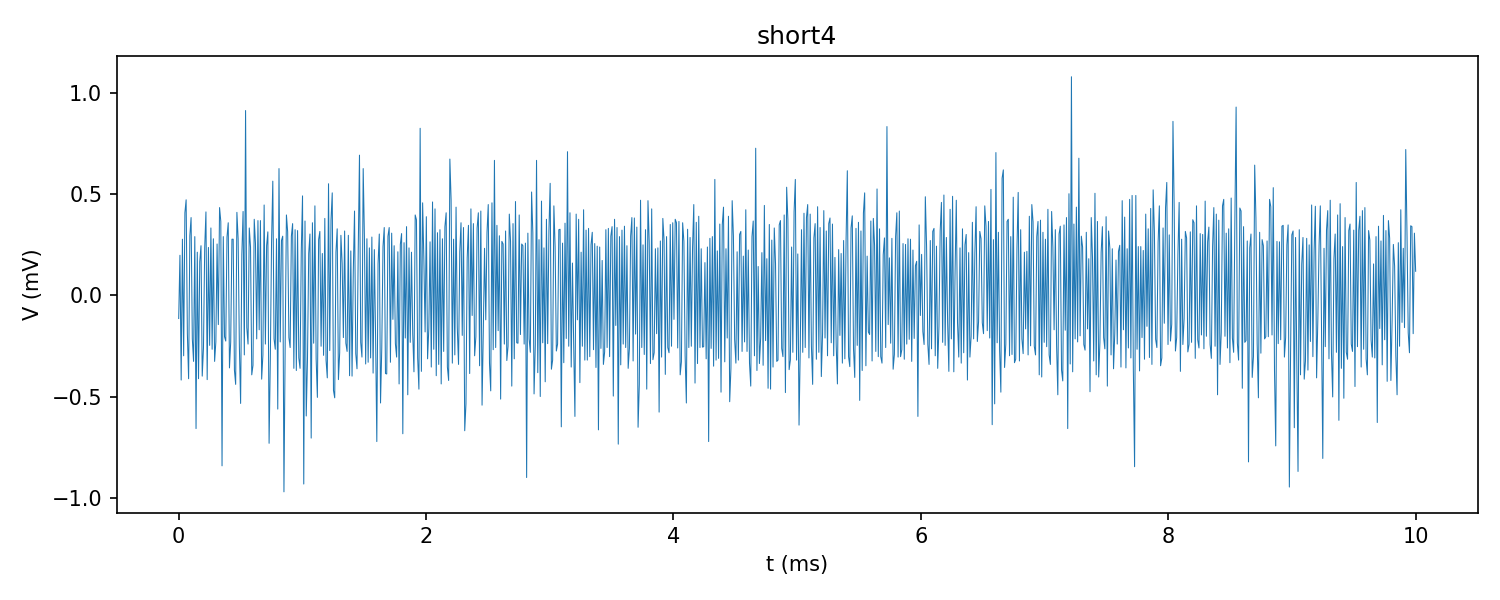
\includegraphics[width=\textwidth]{../images/short4.png}
    \caption{short4}
  \end{subfigure}\\[1em]
  \begin{subfigure}[b]{0.48\textwidth}
    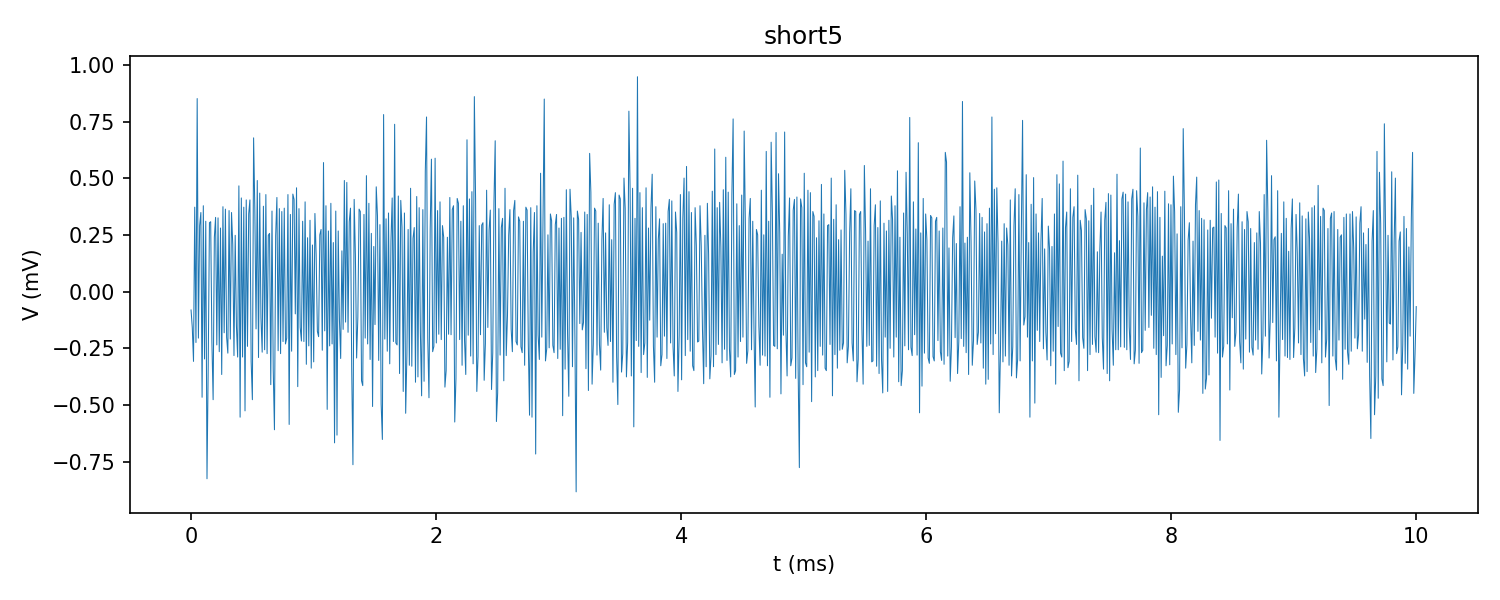
\includegraphics[width=\textwidth]{../images/short5.png}
    \caption{short5}
  \end{subfigure}
  \caption{Individual $V(t)$ traces for short cable measurements.}
\end{figure}

% ============================================================
\newpage
\section*{Team Member Roles}
% ============================================================

\begin{table}[H]
  \centering
  \begin{tabular}{ll}
    \toprule
    {Name} & {Role} \\
    \midrule
    \placeholder{Student 1} & \placeholder{Role description} \\
    \placeholder{Student 2} & \placeholder{Role description} \\
    \placeholder{Student 3} & \placeholder{Role description} \\
    \bottomrule
  \end{tabular}
\end{table}

\end{document}
